\documentclass[../Final.tex]{subfiles}
\begin{document}

This section presented scenario model for collision simulation. 
Scenario was defined including involved ships and configuration during impact. Setting and instrument for numerical calculation was described in following paragraph. 

\begin{figure*}[h]
    \centering
    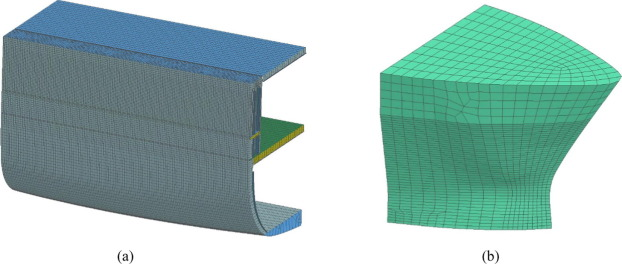
\includegraphics[width=\textwidth]{fig1.jpg}
    \label{fig1}
    \caption{Involved ships for collision analysis: (a) struck ship, and (b) striking ship.}
\end{figure*}

\subsection{Geometry of involved ships}

This work considered 85 m passenger ship as the struck ship or it would be the target of penetration by other ship. 
In other hand, larger cargo ship with size 144 m in length was selected to be the striking ship or the ship that would penetrate the struck ship. 
The detail dimension for both ships are presented in Table 1. Ship models of the struck and striking ships are presented in \hyperref[fig1]{Figure 1}. 
As briefly stated in previous section, the struck ship had different structural configuration on side part of its hull. Double hull spaces with 1.5 m and 3.5 m in width were used in the analyses. 
The illustration and scantling data of the struck ship are presented in \ref{fig2} and \ref{fig3}. 

\subsection{Collision scenario}

Side collision was selected to be implemented as fundamental scenario in present work. 
In this situation, the striking ship penetrated side hull of the struck ship with coming angle 90 degrees or in perpendicular position. 
Main parameters were taken from structural level as different double hull spaces of the struck ship would be the target, and mechanical character­istic and configuration, including strength magnitude, 
failure strain, and hardening type had been selected as parameters in material level. Detail description regarding these configurations are presented consecutively in Table 2. 

\begin{figure}[h]
    \centering
    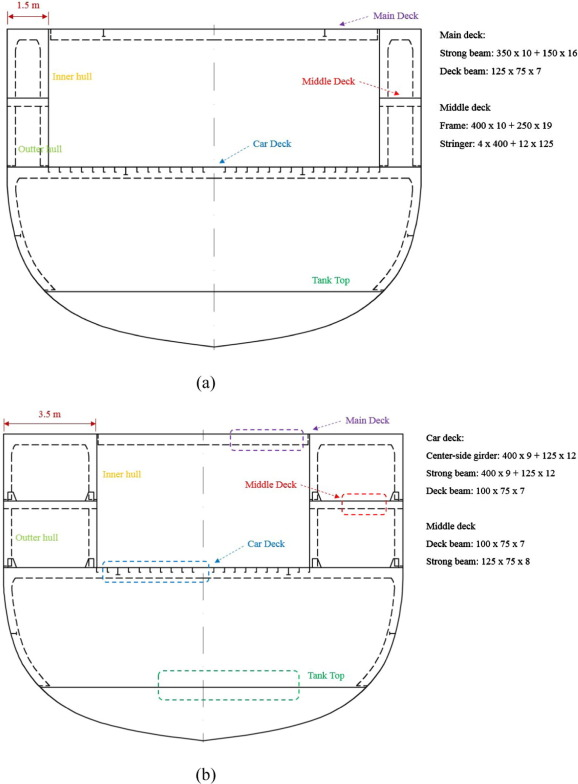
\includegraphics[width=\columnwidth]{fig2.jpg}
    \label{fig2}
    \caption{Configurations of double hull structure: (a) 1.5 m and (b) 3.5 m.}
\end{figure}

\subsection{Setting for numerical calculation}

The numerical calculation would be conducted by ANSYS LS­DYNA \cite{ansys2017user} to perform defined collision scenario and produce structural behaviour during and after collision. 
In this process, the struck ship was defined as deformable structure, and rigid­body characteristic was applied in the striking ship. 
On both of models, plastic-kinematics material which the yield criterion is presented in Eqs. (9) and (10), was implemented together with element formulation Belytschko-Tsay. 
This formulation was considered as it was evidenced by previous author that this formulation type could produce faster results than other options in simulation setting \cite{bae2016study}. 
Meshing size for each ship was given different treatment. The struck ship which was defined as deformable structure, was given meshing size according to rec­ommendation of Tornqvist and Simonsen \cite{toernqvist2004safety}
as well as Alsos and Amdahl \cite{alsos2007resistance}, who indicated that in order to capture local deformation pattern, the size should be given within range of the element-length-to-thickness (ELT) ratio 5–10.


%%Ecuations
\begin{flalign}
    &\sigma_{y} =\left[1+\left(\frac{\varepsilon}{C}\right)^{\frac{1}{P}}\right]\left(\sigma_{0}+\beta E_{p} \varepsilon_{p}^{e f f}\right)& \label{eq9} \\[12pt]
    &E_{p} =\frac{E_{\mathrm{tan}} E}{E-E_{\mathrm{tan}}}& \label{eq10}
\end{flalign}

\begin{figure}[h]
    \centering
    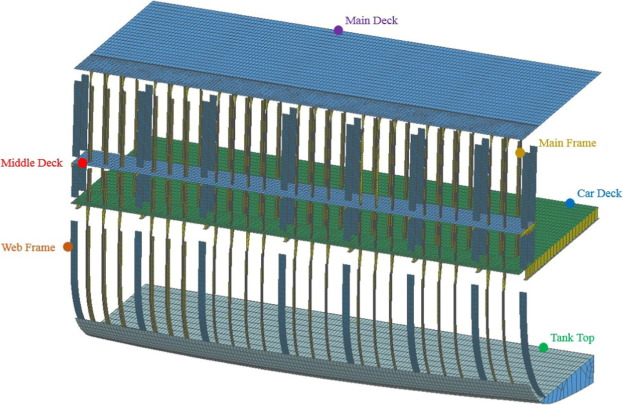
\includegraphics[width=\columnwidth]{fig3.jpg}
    \label{fig3}
    \caption{Structure of the struck ship. Side shell is removed to show transverse and longitudinal components.}
\end{figure}


\begin{table}
    Table 2 Detail of scenario models. \\
    \begin{tabular}{llll}
    \hline 
    Parameters & Impact scenario model & \\
    \hline 
    Structural & Double hull & Space width (m) & $1.50$ \\
    & & & $3.50$ \\
    Material & Strength & Yield - Ultimate & $180-325$ \\
    & & strengths (MPa) & $205-380$ \\
    & & & $430-605$ \\
    & & & $480-800$ \\
    & Failure & Failure strain & $0.1$ \\
    & & & $0.2$ \\
    & & & $0.3$ \\
    & Yield surface & Hardening value & 0 \\
    & & & $0.5$ \\
    & & & 1 \\
    \hline
    \end{tabular}
\end{table}



The struck ship was applied with size 80–100 mm, while the striking ship which had rigid characteristic, larger mesh with 300–700 mm in size was applied on its model. 
Failure on the struck ship was predicted based on applied material behaviour with strain-dependent characteristic was the main influence on failure mode. 
The involved objects were built using steel material and on contact area friction between steels was taken into consideration. Therefore friction coefficient between mild steel was applied in the analyses. 
In the finite element analysis, displacement of the struck ship was set to be fixed at the centre-line, and fixation was applied on all transverse frame and longitudinal deck in the end of model. 
In this location, axial displacements are restrained. The striking ship, in other hand, moved to the designated target points as presented in Fig. 4 with implemented velocity 12 knots or 6.17 m/s in SI unit. 
All defined scenarios were processed on high-performance computer with 4th Generation Intel Core i7-4790 Processor 4.00 GHz, 16 GB RAM. 

\end{document}